\documentclass[10pt]{beamer}

\usetheme[progressbar=frametitle]{metropolis}
\usepackage{appendixnumberbeamer}

\usepackage{booktabs}
\usepackage[scale=2]{ccicons}

\usepackage{pgfplots}
\usepgfplotslibrary{dateplot}

\usepackage{xspace}
\newcommand{\themename}{\textbf{\textsc{metropolis}}\xspace}

% подключаем кириллицу 
\usepackage[T2A]{fontenc}
\usepackage[utf8]{inputenc}
\usepackage{listings}
\usepackage{graphicx}
\usepackage{hyperref}
\usepackage{chronology}


\title{Metropolis}
\subtitle{A modern beamer theme}
% \date{\today}
\date{}
\author{Matthias Vogelgesang}
\institute{Center for modern beamer themes}
% \titlegraphic{\hfill
\includegraphics[height=1.5cm]{logo.pdf}}





\title{Семинар 0}
\subtitle{Обзор 1-го семестра}
%\date{\small{\jobname}}
%\date{\today}
\author{\texttt{Бирюков Владимир}}
\institute{МФТИ}



\begin{document}

%-=-=-=-=-=-=-=-=-=-=-=-=-=-=-=-=-=-=-=-=-=-=-=-=
%
%	TITLE PAGE
%
%-=-=-=-=-=-=-=-=-=-=-=-=-=-=-=-=-=-=-=-=-=-=-=-=

\maketitle

\begin{frame}[fragile]
\frametitle{Главные идеи первого семестра}
\begin{enumerate}
\item Язык C
\begin{enumerate}
\item Синтаксис языка C.
\item Память и указатели.
\item Сегменты памяти процесса. Стек и куча.
\end{enumerate}
\item Алгоритмы и структуры данных
\begin{enumerate}
\item Сложность алгоритмов. $O(n)$ нотация.
\item Основные структуры данных: массив, список, дерево.
\end{enumerate}
\end{enumerate}
\end{frame}


\section{Язык C}


\begin{frame}[fragile]
\frametitle{Память и указатели} 
\begin{center}
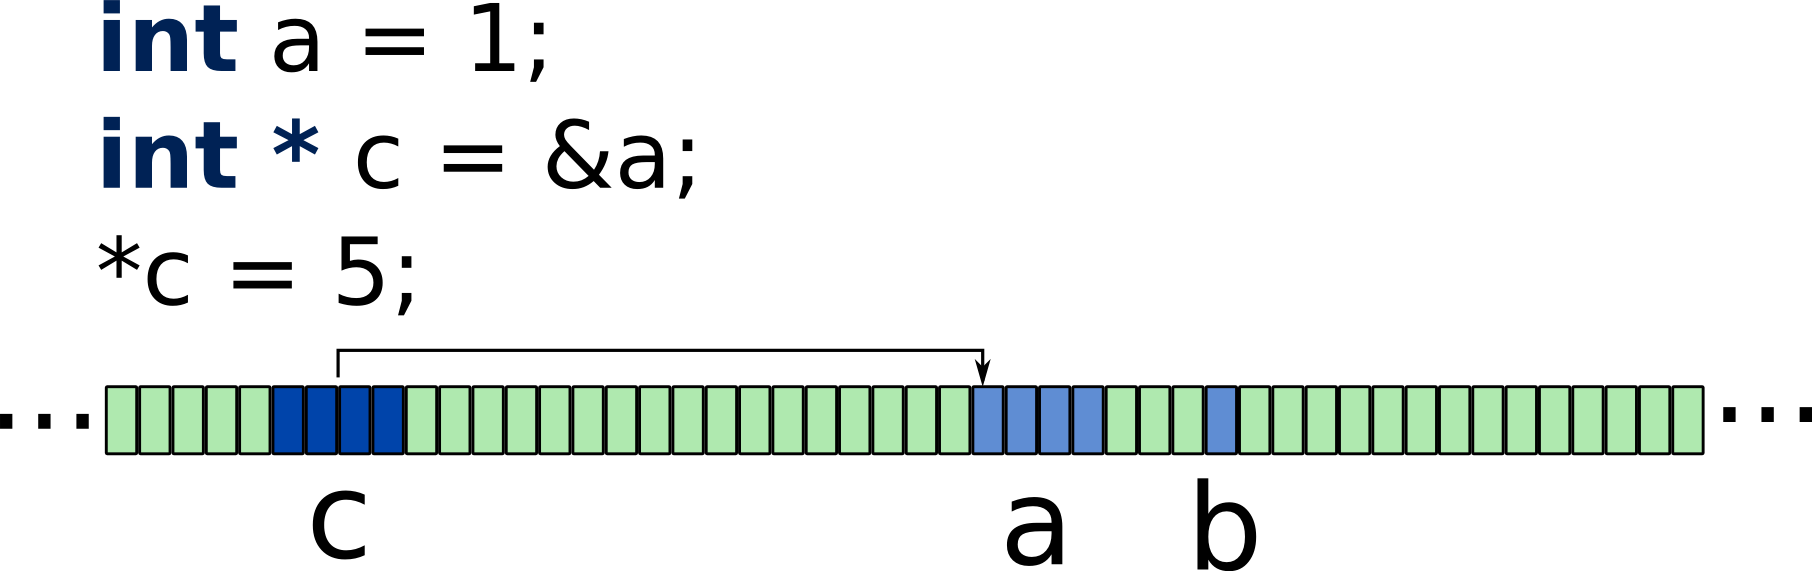
\includegraphics[width=0.95\linewidth]{images/memory_pointer_4.png}
\end{center}
\end{frame}

\begin{frame}[fragile]
\frametitle{Память и указатели. Массив} 
\begin{center}
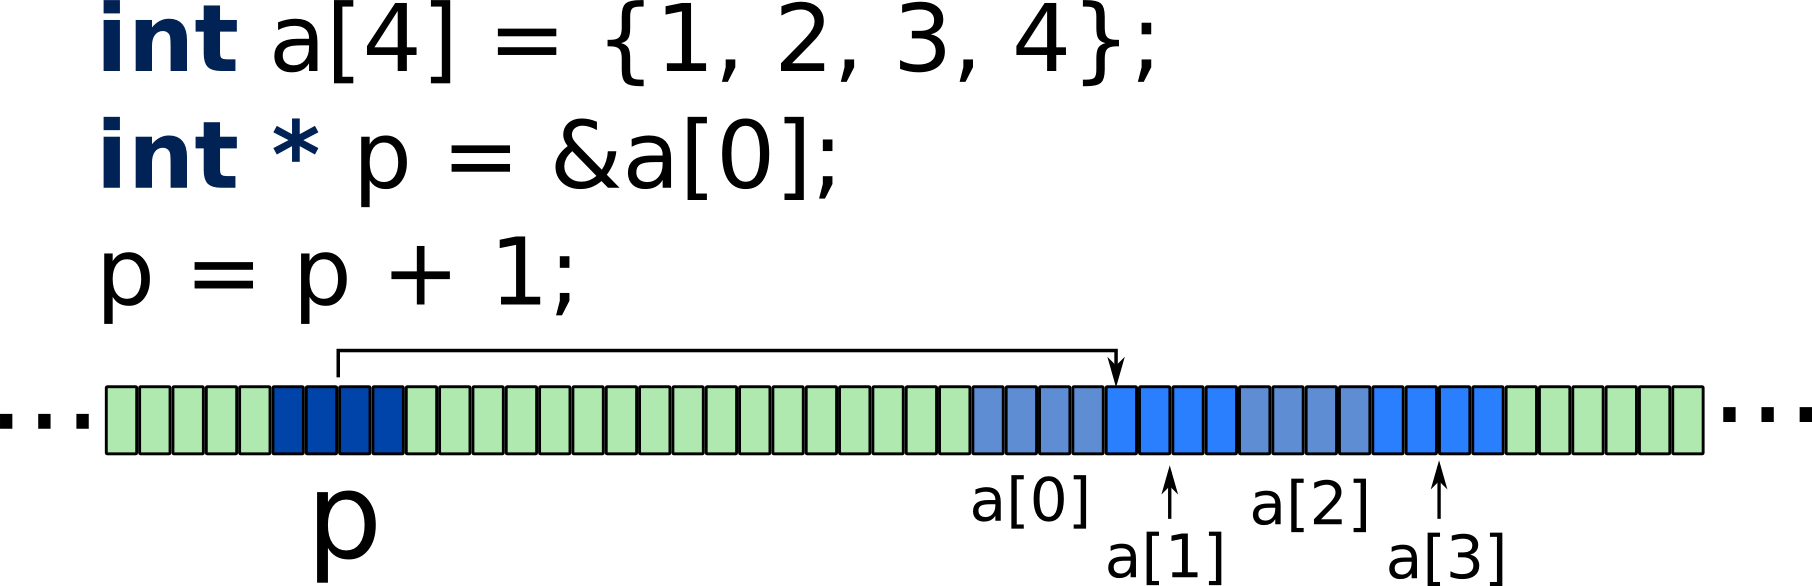
\includegraphics[width=0.95\linewidth]{images/memory_parrays_2.png}
\end{center}
\end{frame}

\begin{frame}[fragile]
\frametitle{Сегменты памяти процесса} 
\begin{center}
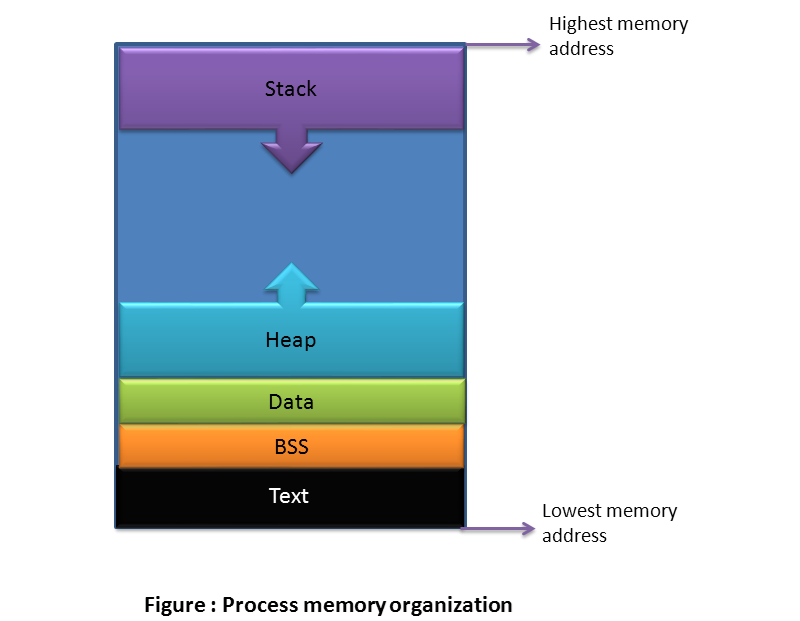
\includegraphics[width=0.95\linewidth]{images/process_memory_organization.png}
\end{center}
\end{frame}

\section{Алгоритмы и структуры данных}

\begin{frame}[fragile]
\frametitle{O-большое} 
\begin{center}
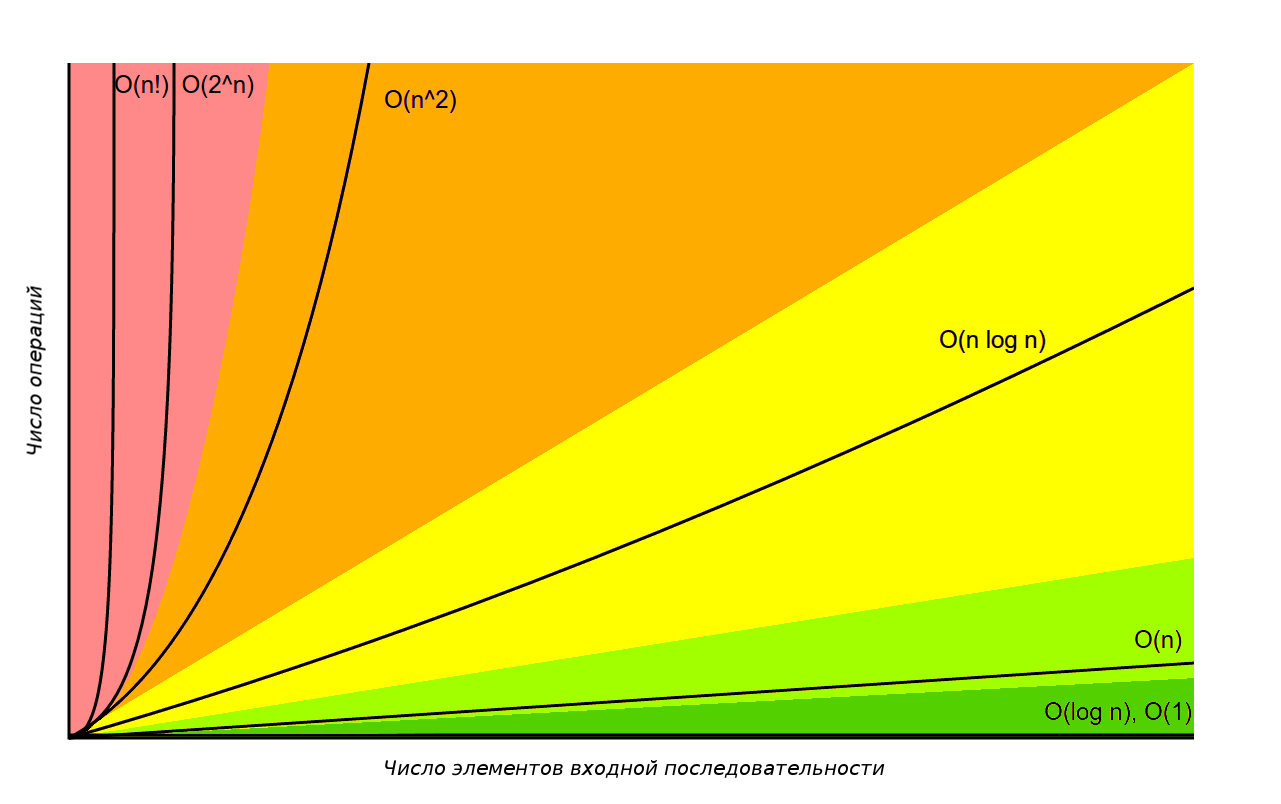
\includegraphics[width=0.99\linewidth]{images/On.png}
\end{center}
\end{frame}

\begin{frame}[fragile]
\frametitle{Алгоритмы сортировки}
\begin{center}
  \begin{tabular}{  l | c }
    Алгоритм сортировки & Сложность(в среднем) \\
    \hline
    Сортировка вставками & O($N^2$)\\
    Сортировка пузырьком & O($N^2$)\\
    Сортировка выбором & O($N^2$)\\
    \hline
    Сортировка слиянием & O($N\log(N)$)\\
    Быстрая сортировка & O($N\log(N)$)\\
    \hline
    Цифровая сортировка &  O($k N$) \\
  \end{tabular}
\end{center}
\end{frame}

\begin{frame}[fragile]
\frametitle{Структуры данных. Связный список} 
\begin{center}
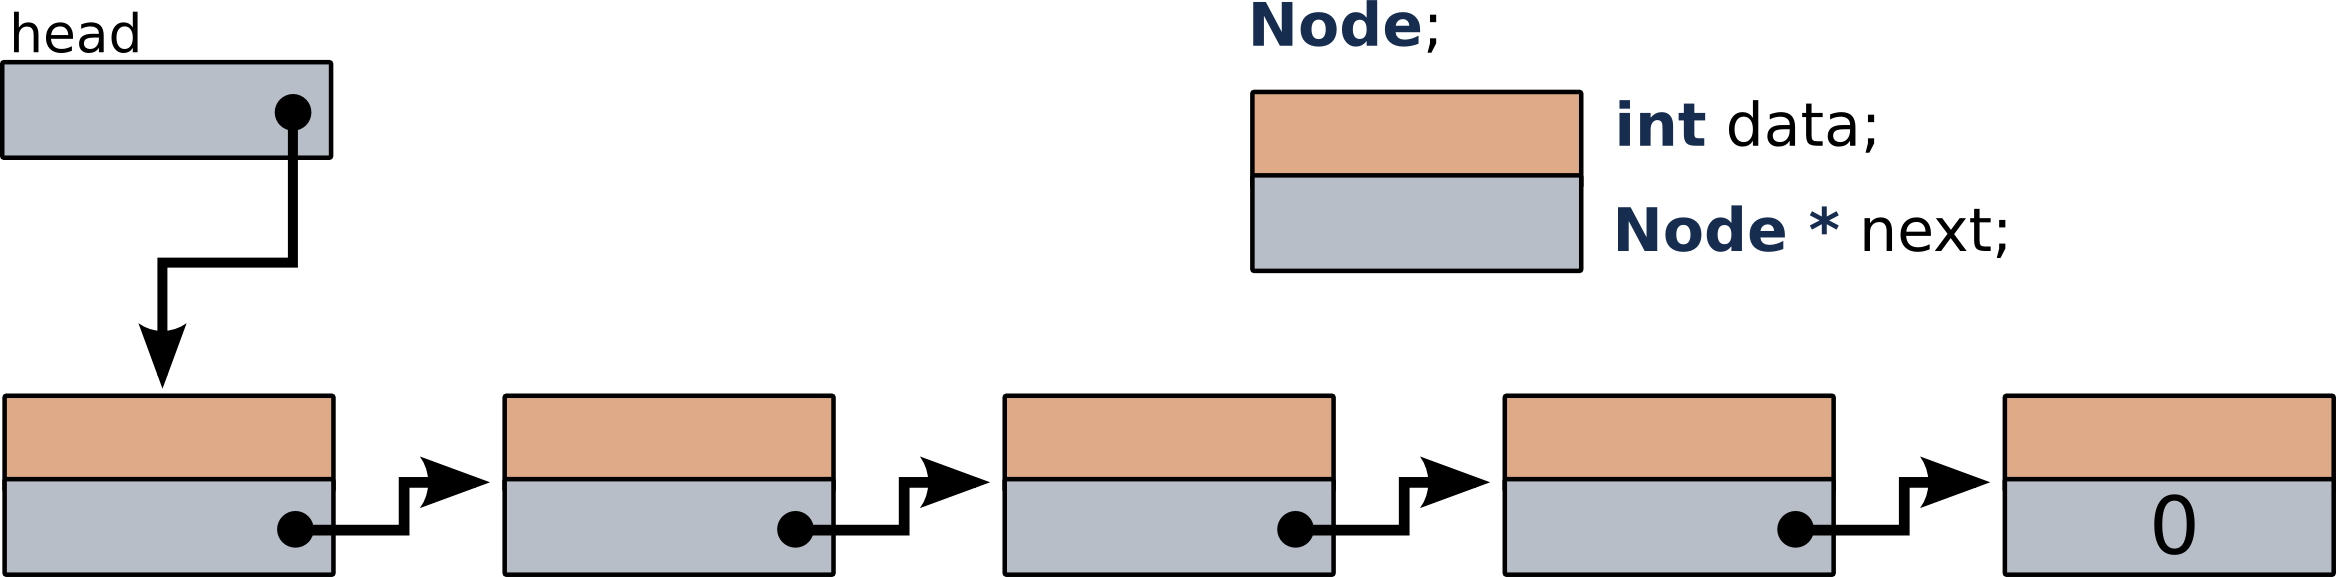
\includegraphics[width=0.99\linewidth]{images/list_initial.png}
\end{center}
\end{frame}

\begin{frame}[fragile]
\frametitle{Структуры данных. Бинарное дерево} 
\begin{center}
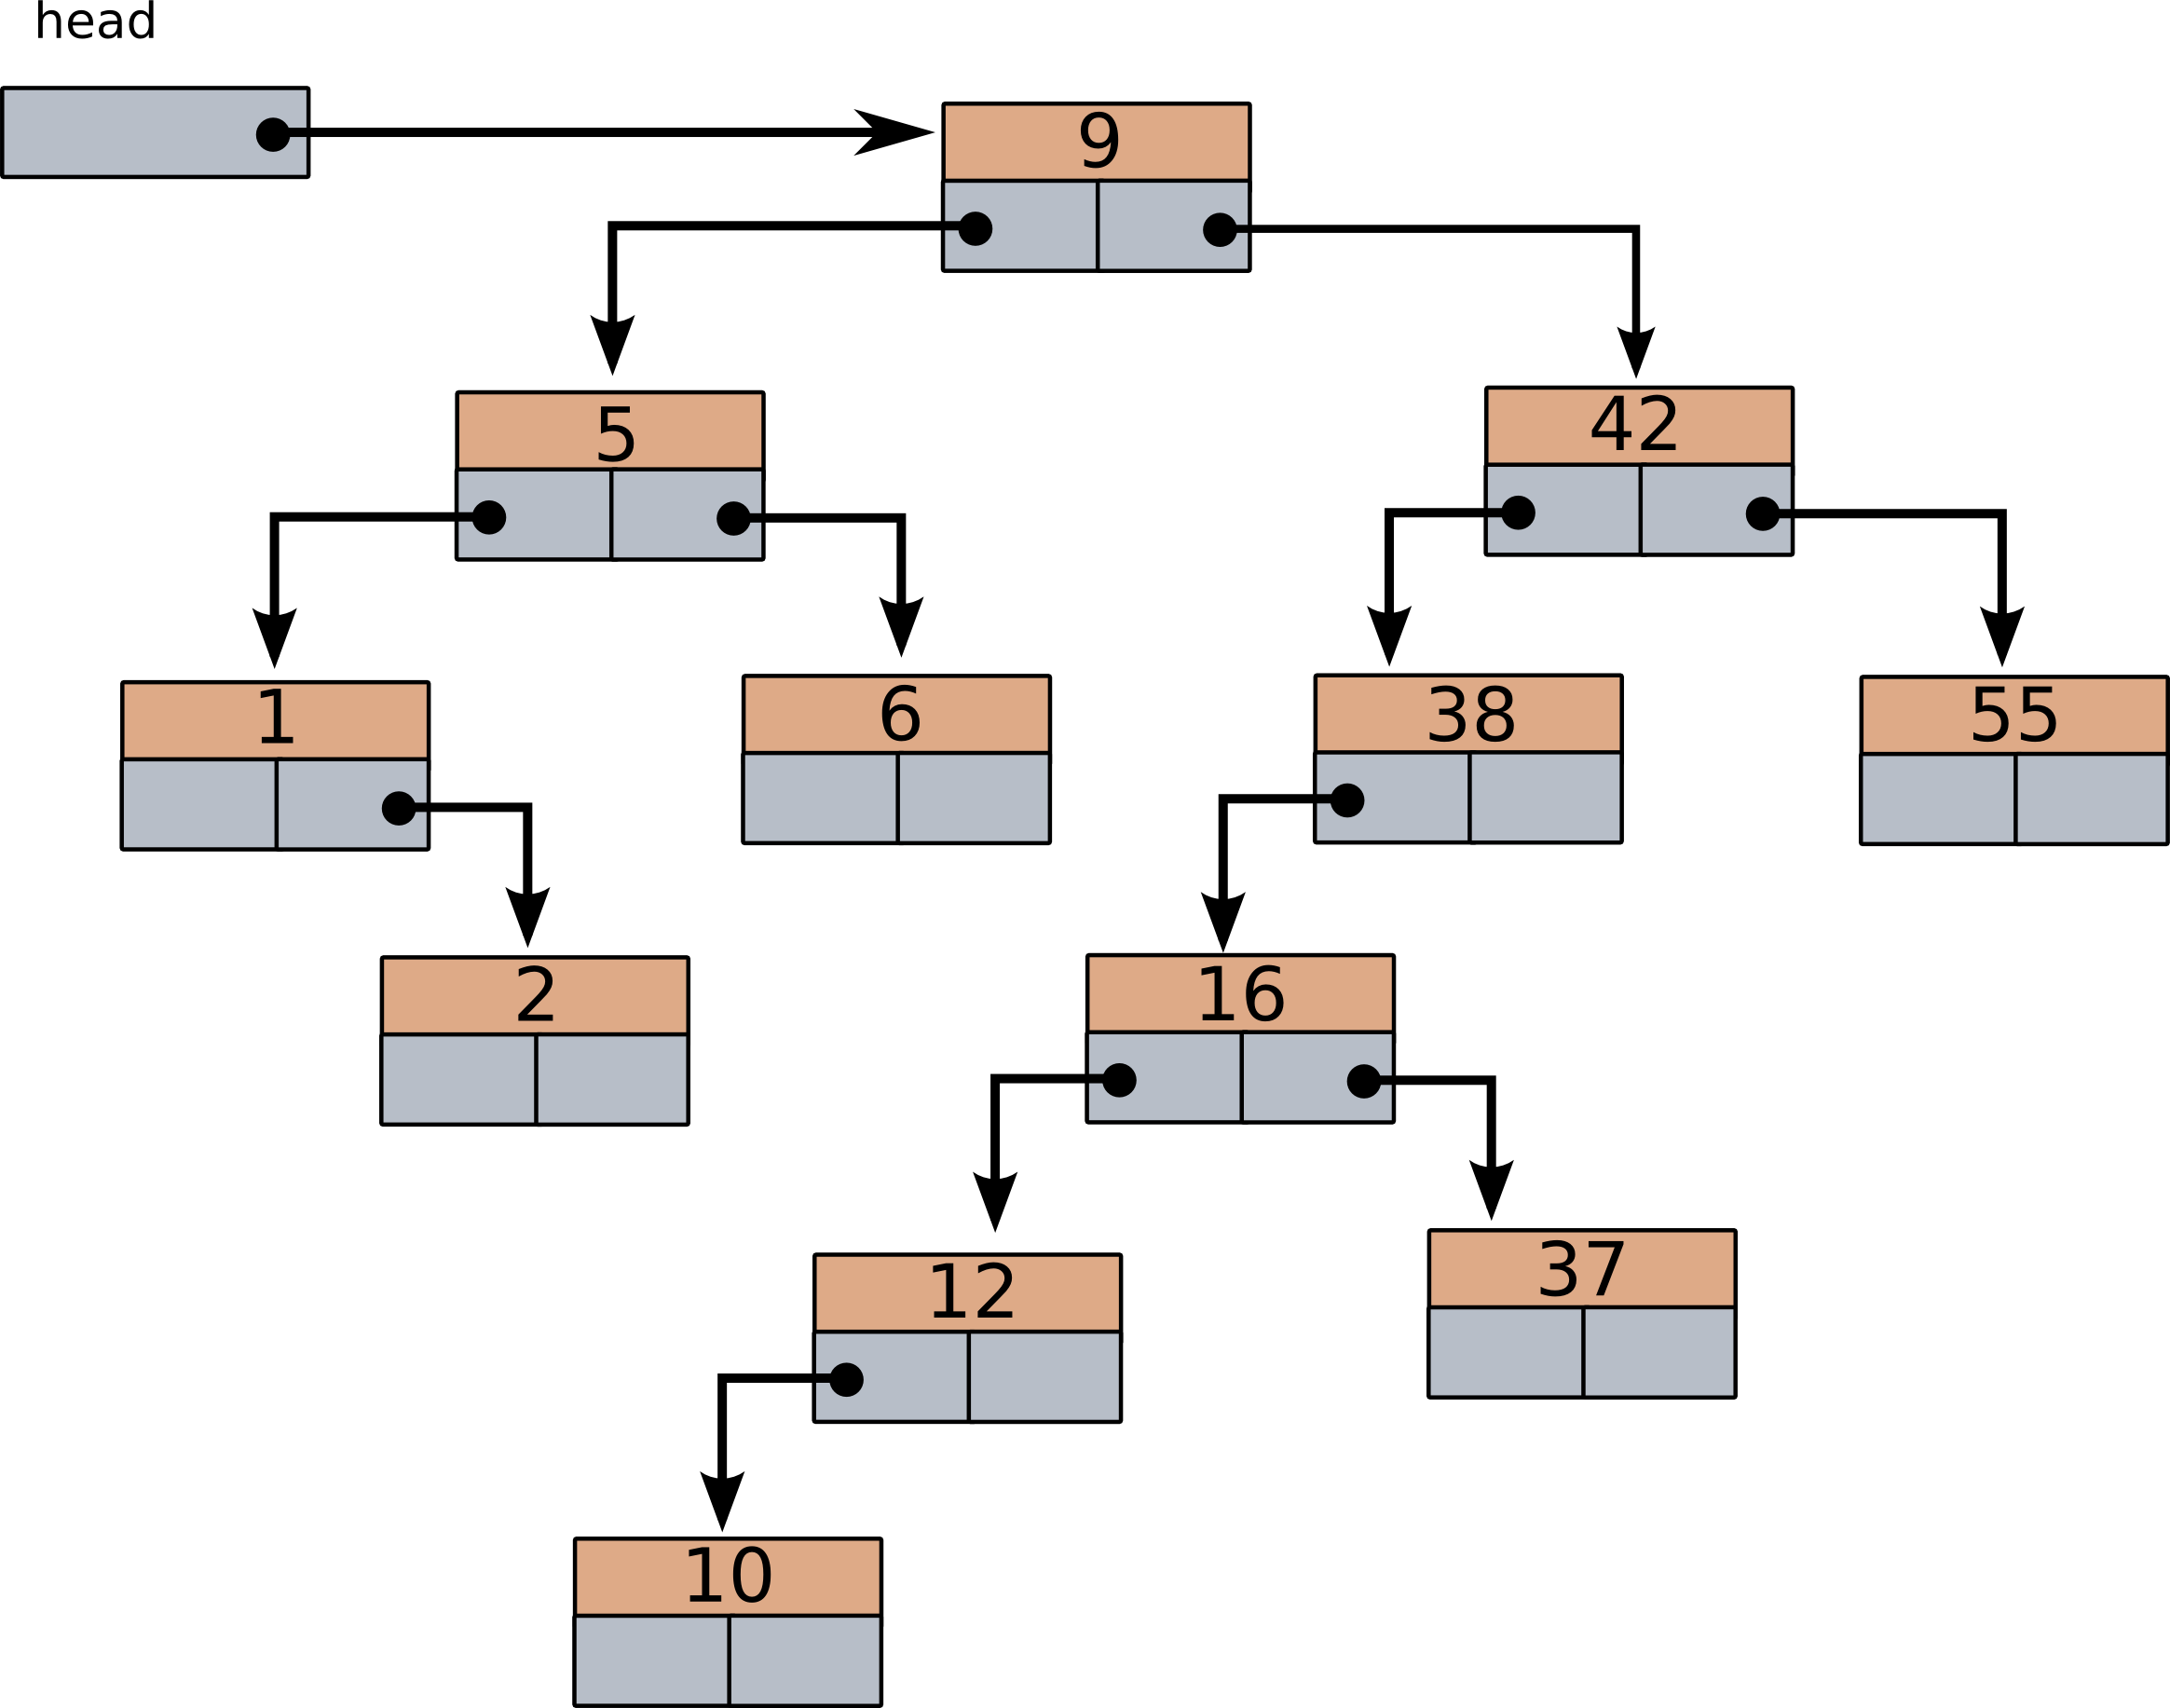
\includegraphics[width=0.95\linewidth]{images/bintree_search_1.png}
\end{center}
\end{frame}


\begin{frame}[fragile]
\frametitle{Операции со структурами данных}
\begin{center}
  \begin{tabular}{  l | c c r }
      & Массив & Список & Бинарное дерево \\
    \hline
    index & $O(1)$ & $O(N)$ & $O(log(N))$ \\
    find & $O(N)$ & $O(N)$ & $O(log(N))$ \\
    insert & $O(N)$ & $O(1)$* & $O(log(N))$ \\
    remove & $O(N)$ & $O(1)$* & $O(log(N))$ \\
    \hline
  \end{tabular}
\end{center}
* если известны указатели на данный и предыдущий элементы.
\end{frame}

\section{Новая тема: Раздельная компиляция}

\begin{frame}[fragile]
\frametitle{Компилируемый язык} 
Язык C является компилируемым языком программирования \\
Компиляция -- преобразование текста программы(исходного кода) в машинный код. \\
\quad\\
Зачем разбивать программу на файлы?
\begin{enumerate}
\item С небольшими файлами удобнее работать
\item Ускорения повторной компиляции при небольших изменениях
\item Структуирование кода
\end{enumerate}

\end{frame}

\begin{frame}[fragile]
\frametitle{Общая схема сборки программы} 
\begin{center}
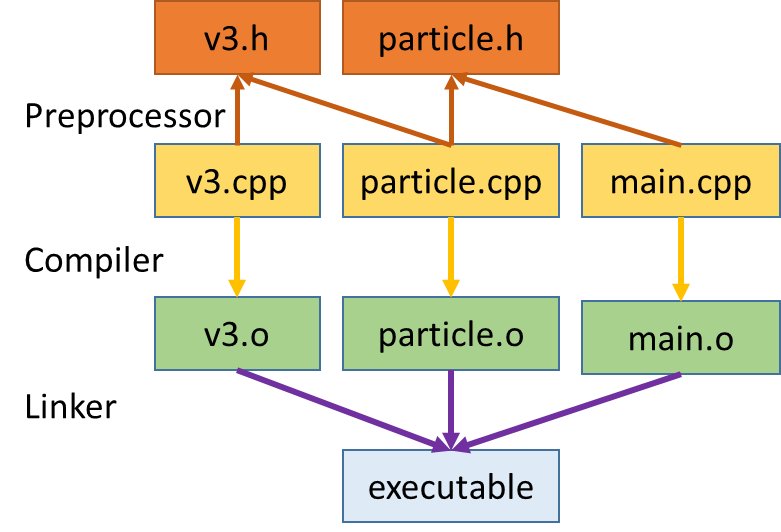
\includegraphics[width=0.95\linewidth]{images/separate_compilation_linking.png}
\end{center}
\end{frame}





\end{document}